\section{Vergleich verschiedener Algorithmen}\label{s.Ergebnisse}\raggedbottom

\subsection{Wahl der Parameter}

\subsubsection{Vergleich der drei Euklid Varianten}\label{s.keuclid}
\begin{figure}[htbp!]
	\centering
	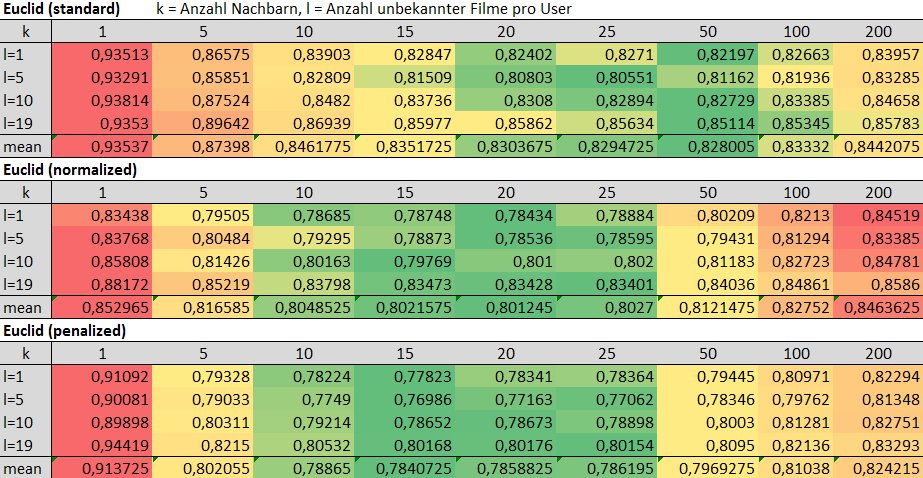
\includegraphics[width=1\linewidth]{ErrorEuclid}
	\caption{MAE im Euklid Algorithmus in Abhängigkeit der Parameter}
	\label{fig:ErrorEuclid}
	
\end{figure}
Die Werte sind mit einer Farbskala von Rot über Gelb nach Grün je Zeile formatiert, um den maximalen Fehler (rot) und den minimalen Fehler (grün) besser erkennen zu können.\\\\
Wie man an den Tabellen sehen kann, verbessert die Normalisierung den Standard-Euklid-Algorithmus aus \autoref{euclid} . Eine stärkere Verbesserung wird jedoch durch die eingebaute Strafe erzielt. Mit den Parametern $k = 15$ und der Strafe kann der Fehler minimiert werden. In den folgenden Vergleichen werden immer diese Parameter benutzt.
\clearpage

\subsubsection{Wahl von $k$ bei den kNN im Pearson Algorithmus}\label{s.kpearson}
\begin{figure}[htbp!]
\centering
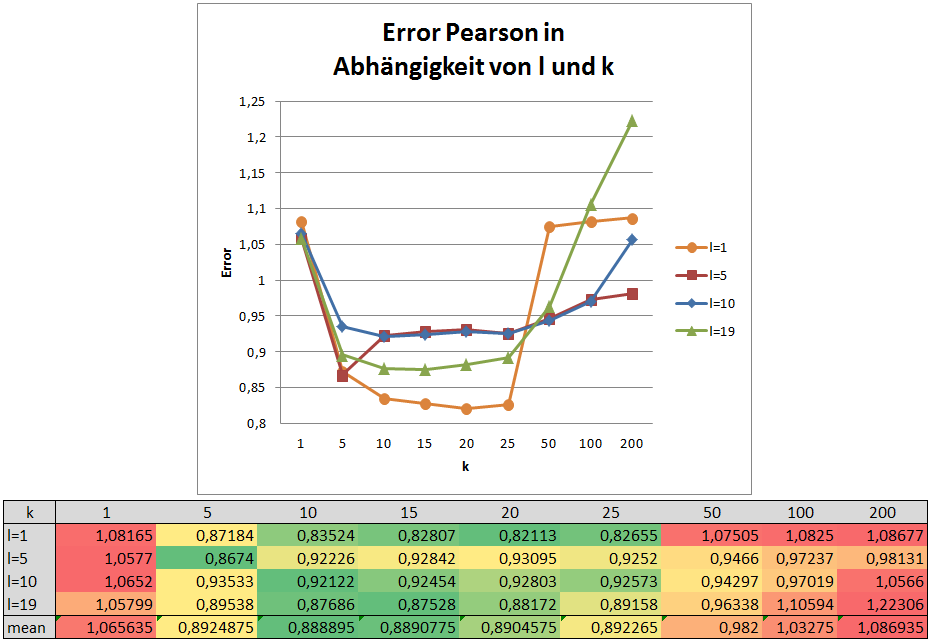
\includegraphics[width=1\linewidth]{ErrorPearsonk}
\caption{MAE im Pearson Algorithmus in Abhängigkeit der Parameter }
\label{fig:ErrorPearsonk}
\end{figure}
Eine Wahl von $k = 10$ nächsten Nachbarn optimiert den Pearson Algorithmus. Im Szenario $l = 1$ zeigt der Algorithmus seine Stärken. Wenn viele Informationen vorhanden sind, können mit dem Pearson Algorithmus gute Bewertungen vorhergesagt werden. Wenn man die mittleren Szenarien $l = 5$ und $l = 10$ mit $l = 19$ vergleicht, fällt auf, dass das letzte Szenario am besten abschneidet. Da hier 19 Fehler berechnet und gemittelt werden. Im Fall $l = 5$ werden nur fünf Fälle verglichen, dadurch entsteht im Mittel eine größere Abweichung zwischen der Vorhersage und der tatsächlich abgegeben Bewertung.
\clearpage

\subsubsection{Wahl von $k$ bei den kNN im Floyd Warshall Algorithmus}\label{s.kflowar}
\begin{figure}[htbp!]
\centering
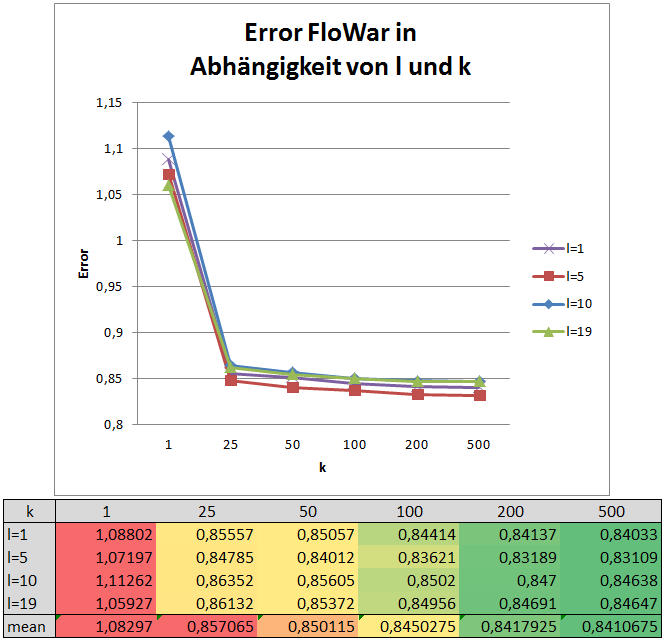
\includegraphics[width=1\linewidth]{ErrorFloWark}
\caption{MAE im Floyd Warshall Algorithmus in Abhängigkeit der Parameter}
\label{fig:ErrorFloWark}
\end{figure}
Man sieht in \autoref{fig:ErrorFloWark}, dass Floyd-Warshall bei großem $k$ (=200-500) am besten funktioniert. Es wird das Minimum aus den $k$ nächsten Nachbarn und den n nächsten Nachbarn, die den aktuell zu bewertenden Film überhaupt bewertet haben, genommen, um das zu erwartete Rating zu ermitteln. Dies tendiert gegen den Durchschnittswert aller User, die die fehlenden Items bewertet haben. Somit ist der FW-Algorithmus fast gleichzusetzen mit dem Itemmean.
\clearpage

\subsubsection{Wahl von $a$ beim LUS-GUS Algorithmus}\label{s.alugu}

\begin{figure}[htbp!]
\centering
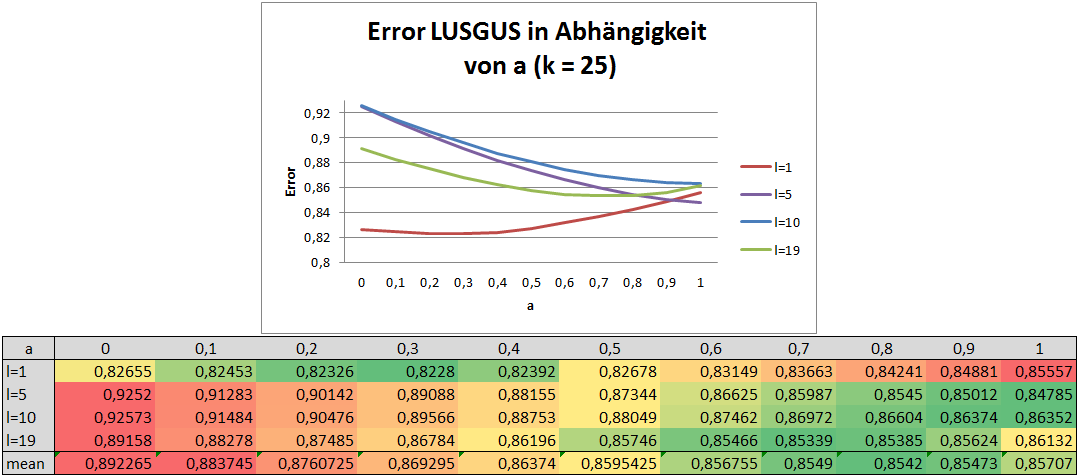
\includegraphics[width=1\linewidth]{ErrorLUSGUSa}
\caption{MAE im LUS-GUS Algorithmus in Abhängigkeit der Parameter}
\label{fig:ErrorLUSGUSa}
\end{figure}
\FloatBarrier
Sind viele Informationen über die User gegeben ( $l = 1$ ) kann der LUS-GUS die Stärken des Pearson Algorithmus ausspielen. Es finden sich gute direkte Nachbarn die sehr ähnlich sind. Trotzdem kann das Wissen aus dem Floyd-Warshall-Algorithmus über indirekte Nachbarn den MAE weiter minimieren. Optimal wird das Rating zu 80\% aus dem FW und zu 20\% aus dem Pearson Algorithmus ermittelt. Ist nicht viel über die User bekannt, wird der Graph-Algorithmus bedeutender. Informationen die aus einer Kombination aus mehreren User entstehen, erzielen in diesem Fall bessere Ergebnisse.


\subsection{Auswertung der Fehlerberechnung}\label{s.auswertung}
Neben den 6 genannten Algorithmen habe ich noch 3 weitere Algorithmen für den Vergleichstest implementiert. Der einfachste, Random, erzeugt einen randomisierten Float zwischen $[1,5]\subset \mathbb{R}$. Usermean $\bar{R}^{user}_{u}$ kalkuliert den Durchschnitt des Users, der gerade betrachtet wird. Itemmean $\bar{R}^{item}_{i}$ berechnet die durchschnittliche Bewertung aller User des Items, das gerade im Fokus ist (s. \autoref{definition}). 
Gegen diese 3 simplen Algorithmen werden die MAE der 6 oben beschriebenen Funktionen gemessen. Wobei wieder alle 4 Szenarien bezüglich des Parameters $l$ betrachtet werden.\\

\begin{figure}[htbp!]
\centering
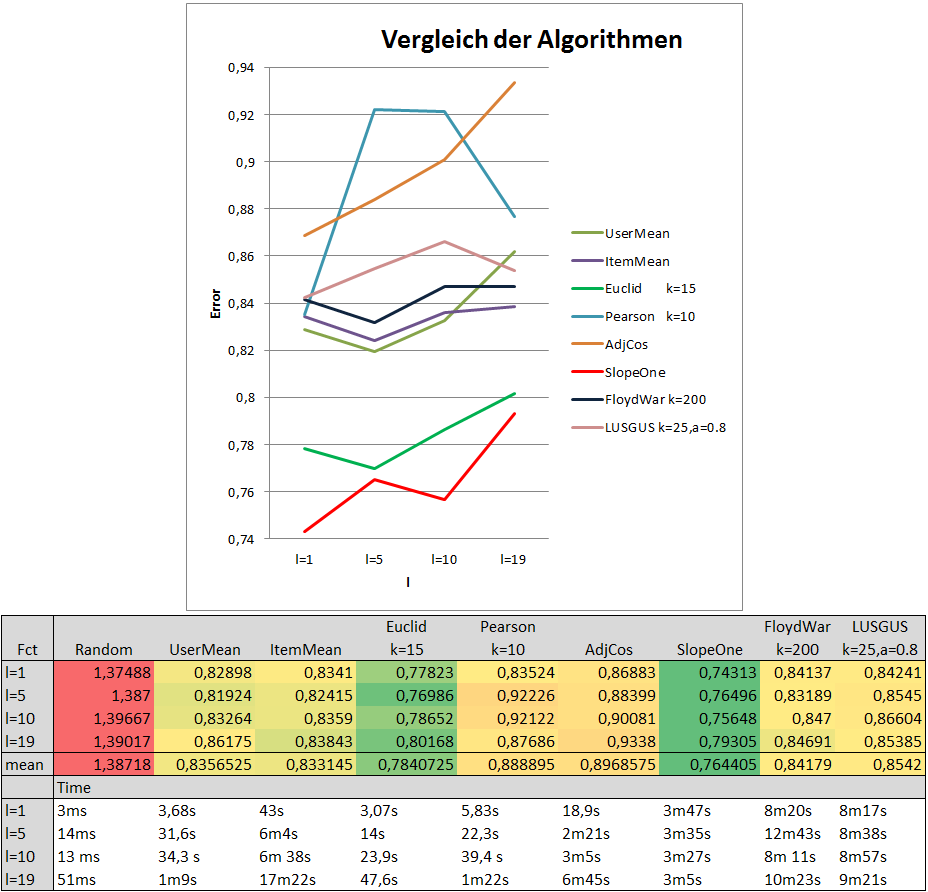
\includegraphics[width=1\linewidth]{Vergleich}
\caption{MAE Vergleich aller Algorithmen}
\label{fig:Vergleich}
\end{figure}
\FloatBarrier
Die Laufzeiten dienen als relativer Vergleich zwischen den Algorithmen. Die Daten sind in einer Hashmap gespeichert und es wird nur ein Kern der CPU ausgelastet. Durch andere Implementierungen und andere PC-Setups können die Zeiten variieren.\\
Usermean und Itemmean erzielen im Vergleich kein schlechtes Ergebnis, zählen sogar laut MAE mit zu den besten Algorithmen. Sie sind aber für Vorhersagen nicht verwendbar. Bei Usermean bekommt jedes unbekannte Item das gleiche Rating. So können keine Vorschläge gemacht werden, die aus dem besten Rating resultieren. Bei Itemmean werden die Vorlieben des Users komplett ignoriert. Pearson erkennt sogar Ähnlichkeiten in relativen Abweichungen und kommt somit mit einem geringem $k$ im k-Nearest-Neighbors aus. Das genaue Gegenteil ist bei Floyd-Warshall der Fall. Der sehr groß eingestellte Parameter $k$ führt dazu, dass FW ähnlich wie Itemmean die bekannten Informationen über den User vernachlässigt. Da mit dem Itemmean eine bessere durchschnittliche Abweichung erzielt wird, als über die entdeckten Pfade zu anderen User. Dennoch kann FW den Pearson Algorithmus verbessern. Die Kombination beider Algorithmen im LUSGUS-Verfahren erzielt leicht bessere Ergebnisse, ist aber in meinem Test den Mehraufwand an Rechenleistung, gegenüber Pearson, nicht Wert. Adjusted Cosine Similarity ist in diesem Test nicht sehr erfolgreich. Obwohl es mit der gleichen Score arbeitet wie der PCC und dort alle bekannten Informationen über die zwei Items verwendet, können keine guten Vorhersagen erzielt werden. Der Algorithmus mit dem euklidischen Abstand und Strafe schneidet sehr gut ab und hat dazu sehr kurze Berechnungszeiten. Bessere Vorhersagen erzielt man nur mit dem Item-basierten Algorithmus Slope One. Die absolute durchschnittliche Differenz zwischen den Items verwendet alle verfügbaren Informationen aus dem Datensatz. Neben den Differenzen zwischen allen Items muss auch noch eine Frequenzmatrix gespeichert werden. Neue Informationen können dadurch ohne großen Rechenaufwand in die Abstandsmatrix eingearbeitet werden. Die Vorberechnungen im SlopeOne machen ca. 30 Sekunden der gesamten Zeit aus.\\
Die Entscheidung welchen Algorithmus man verwenden sollte liegt an vielen Faktoren. Hat man sehr viele User auf wenige Items, trumpfen Item-basierte Algorithmen auf. Die Item-Item-Matrix hat in diesem Fall kleinere Dimensionen. User-basierte Verfahren müssen erst die Abstände zu allen anderen Nutzern berechnen um die ähnlichsten Nutzer zu finden. Ist das Verhältnis User zu Items anders herum, können User-basierte Algorithmen eine Alternative sein. Alle User zu betrachten ist unter diesen Umständen eventuell schneller oder nicht so speicherintensiv wie eine sehr große Item-Item-Matrix. Generell wird eine Kombination aus mehreren Verfahren in der Praxis die besten Ergebnisse erzielen. Demographische Informationen aus dem Userprofil oder Tags bieten weitere Ansätze um Distanzen zwischen User oder Items zu erstellen. \\
Zudem haben alle Algorithmen Schwierigkeiten damit einem neuem User Vorschläge zu bereiten, da sein persönlicher Geschmack noch nicht bekannt ist. Neue Items zu integrieren erfordert ebenfalls andere Ansätze.
\begin{figure}[htbp!]
	\centering
	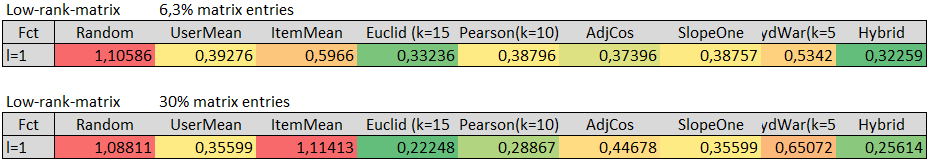
\includegraphics[width=1\linewidth]{bilder/lowrank}
	\caption{MAE Vergleich mit einer Matrix mit niedrigem Rang}
	\label{fig:LowRankMatrix}
\end{figure}
\FloatBarrier
Bei der Konstruktion mit niedrigem Rang erkennt man, dass die User-basierten Algorithmen richtig gut werden. Das ist aber auch zu erwarten, denn die User ähneln sich sehr stark, da sie alle aus einer Kombination aus dreißig Basis-User entstanden sind. In diesem Szenario kann das Euklid-Verfahren den sonst starken Slope-One von der Top Position verdrängen. Die Bewertungen wurden zufällig erstellt, dadurch können auch keine Ähnlichkeiten zwischen den Filmen entstehen. Dies wertet die Item-basierten Algorithmen zusätzlich ab.\\
Einen Vergleich zu der realen Datenbank von MovieLens kann man nur mit Vorsicht tätigen. Wenn man die Histogramme der beiden Matrizen betrachtet, wird klar, dass die Konstruktion der Matrix mit niedrigem Rang nicht sehr nah an die Verteilung der MovieLens-Daten heran kommt.
\begin{figure}[htbp!]
	\centering
	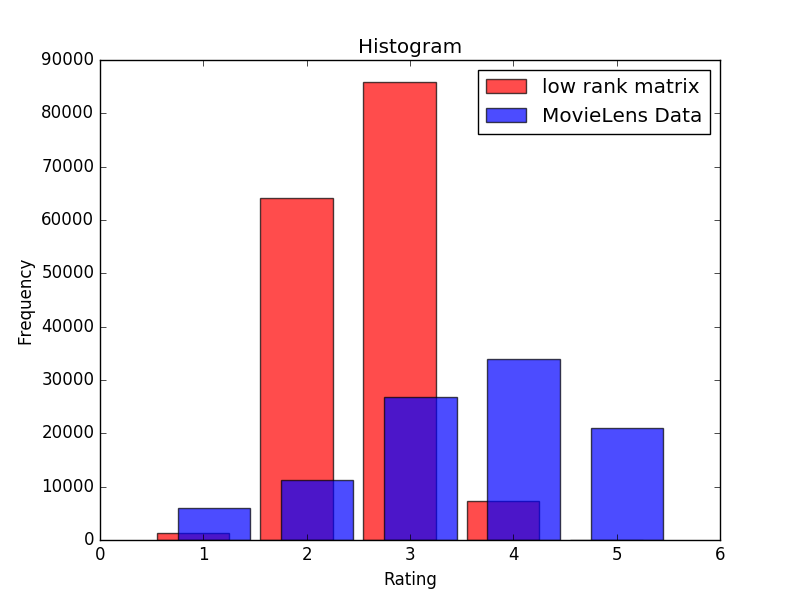
\includegraphics[width=1\linewidth]{histogram}
	\caption{Histogramm Vergleich}
	\label{fig:histogram}
\end{figure}
\FloatBarrier
Beim Versuch die Bewertungen gleichmäßiger zu verteilen zerstört man die lineare Abhängigkeit der Zeilen.

\begin{figure}[htbp!]
	\centering
	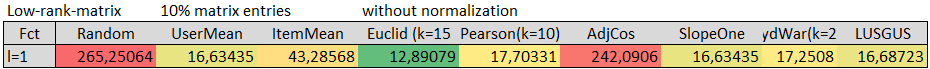
\includegraphics[width=1\linewidth]{lowranknotnorm}
	\caption{MAE Vergleich ohne Normalisierung}
	\label{fig:LowRankMatrixnotnorm}
\end{figure}
\FloatBarrier
In den Daten in \autoref{fig:LowRankMatrixnotnorm} wurde bewusst vermieden, die Bewertungen wieder in den Wertebereich $[1,5]\subset \mathbb{N}$ zu normieren. Dadurch wird die lineare Abhängigkeit der Zeilen nicht zerstört. Diese erzielten Fehler können deshalb nicht mit den anderen Szenarien verglichen werden. Was man aber erkennen kann, dass die User-basierten Verfahren sehr viel besser abschneiden, als der Item-basierte Algorithmus Adjosted Cosine Similarity. Slope One kann auch hier mit den vollen Informationen der Matrix ein sehr gutes Ergebnis erzielen.\\
Abschließend lässt sich keine große Aussage mit diesem zweiten Test erzielen. Die User-basierten Algorithmen sind per Konstruktion sehr gut. Die Item-basierten Verfahren können durch die zufälligen Bewertungen keine Ähnlichkeiten zwischen den Items erkennen. Zusätzlich ist die Verteilung in der Konstruktion weit entfernt von der realen Verteilung der MovieLens-Daten.

\clearpage